\frame{\frametitle{We've run simulations in 2D and 3D with PADDI, and find similar results---except in particular cases with strong shear.}
\setbeamercovered{transparent}
\begin{tabular}{r c c}
	\vtop{\null\hbox{\scalebox{0.7}{\begin{tabular}{r}
		$\rm{Pr}=0.03$ \\
		$\tau=0.3$ \\
		$R_{0}^{-1}=1.1,1.2$ \\
	\end{tabular}}}} &
	\fbox{\vtop{\null\hbox{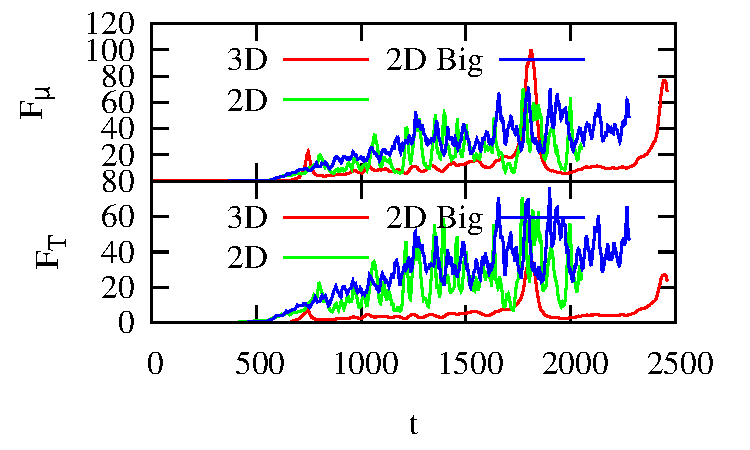
\includegraphics[width=0.35\textwidth]{figs/Pr=0_03_t=0_3_R0-1=1_1.pdf}}}} &
	\fbox{\vtop{\null\hbox{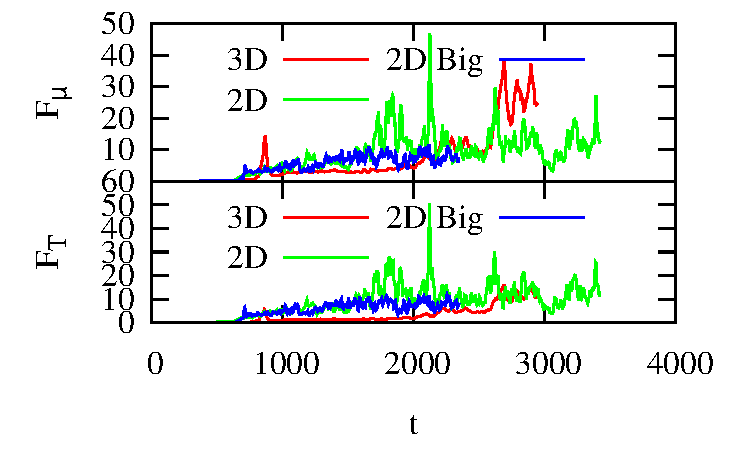
\includegraphics[width=0.35\textwidth]{figs/Pr=0_03_t=0_3_R0-1=1_2.pdf}}}} \\
	\vtop{\null\hbox{\scalebox{0.7}{\begin{tabular}{r}
		$\rm{Pr}=0.01$ \\
		$\tau=0.01$ \\
		$R_{0}^{-1}=1.5,2$ \\
	\end{tabular}}}} &
	\vtop{\null\hbox{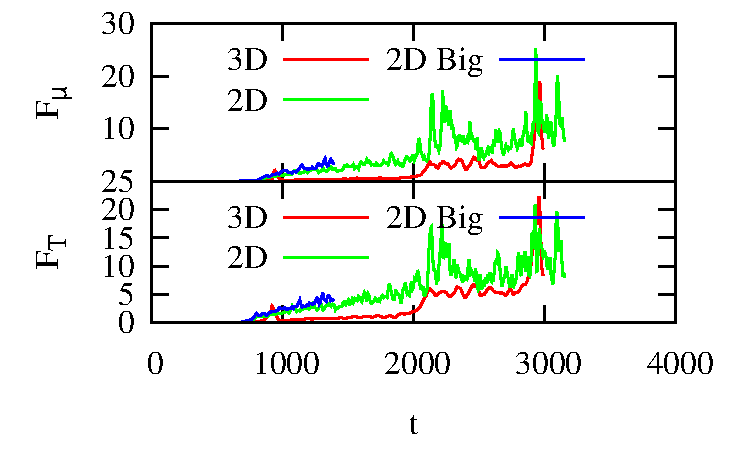
\includegraphics[width=0.35\textwidth]{figs/Pr=0_01_t=0_01_R0-1=1_5.pdf}}} &
	\vtop{\null\hbox{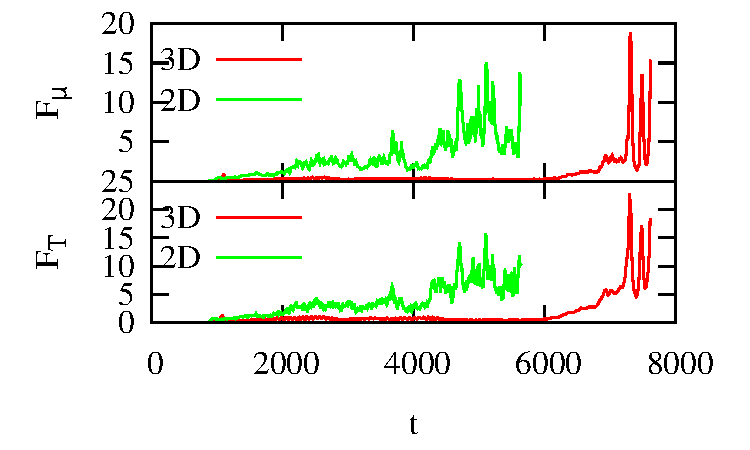
\includegraphics[width=0.35\textwidth]{figs/Pr=0_01_t=0_01_R0-1=2.pdf}}} \\
\end{tabular}
}

\frame{\frametitle{At early stages, the simulations have similar behavior; however, at late stages, large shear dominates the 2D runs.}
\begin{overprint}
	\only<1>{
	\begin{figure}[h]
		\centering
			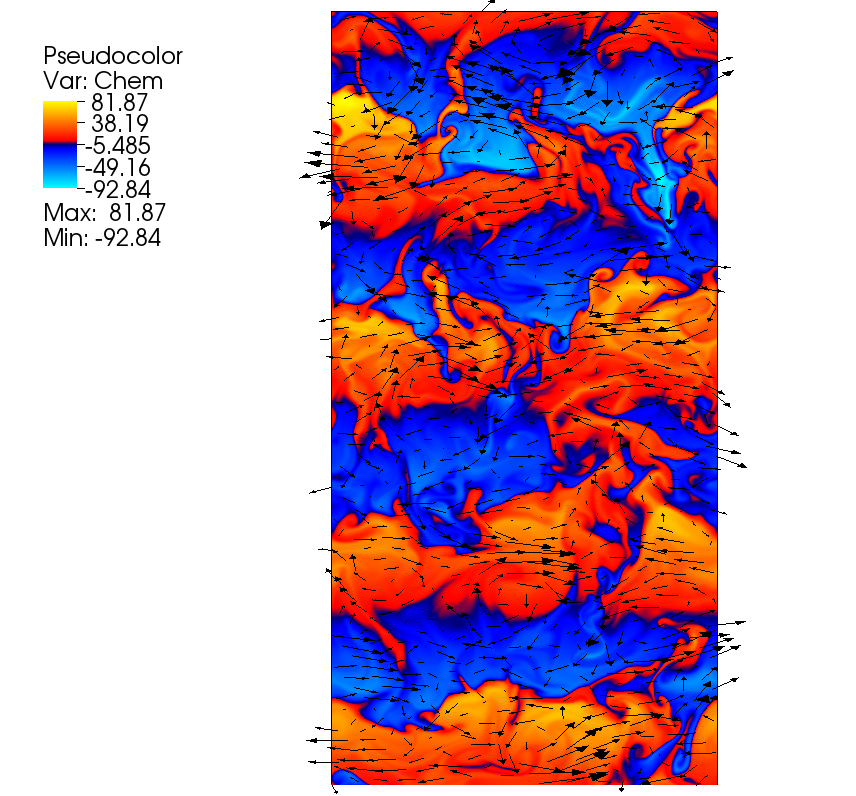
\includegraphics[width=.55\textwidth]{../pngs/movie0003.png}
		\label{fig:pngs_movie0003}
		\caption{$\rm{Pr}=0.3$, $\tau=0.3$, $R_{0}^{-1}=1.15$}
	\end{figure}
	}
	\only<2>{
	\begin{figure}[h]
		\centering
			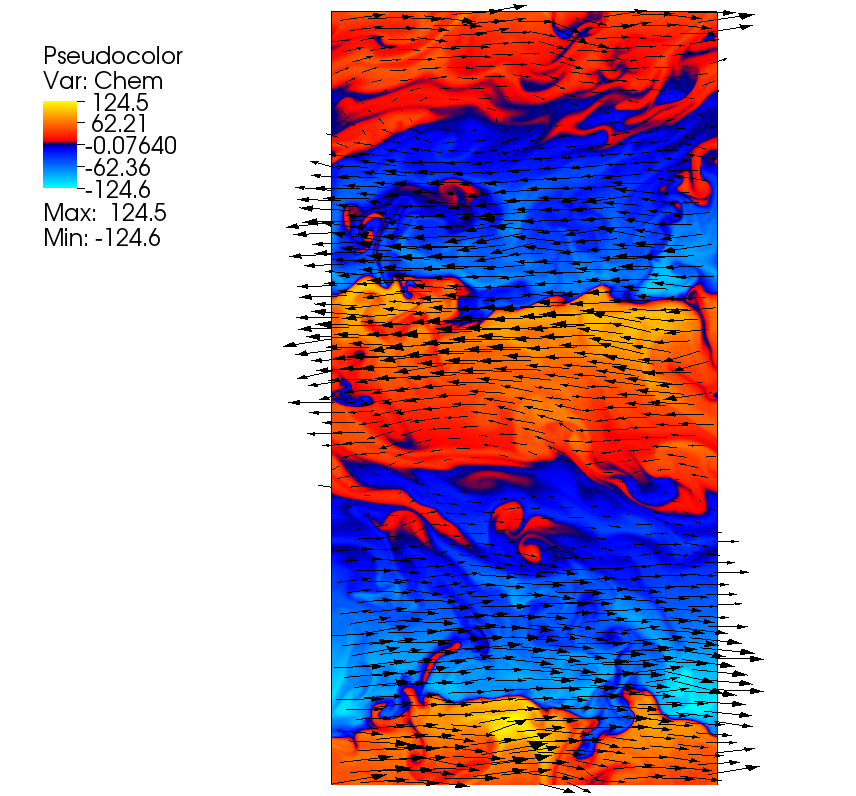
\includegraphics[width=.55\textwidth]{../pngs/movie0014.png}
		\label{fig:pngs_movie0014}
		\caption{$\rm{Pr}=0.3$, $\tau=0.3$, $R_{0}^{-1}=1.15$}
	\end{figure}
	}
\end{overprint}
}

\frame{\frametitle{Fortunately, this problem appears absent in the low viscosity and compositional diffusivity runs at low $R_0^{-1}$.}
\setbeamercovered{transparent}
\begin{tabular}{r c c}
	\vtop{\null\hbox{\scalebox{0.7}{\begin{tabular}{r}
		$\rm{Pr}=0.03$ \\
		$\tau=0.3$ \\
		$R_{0}^{-1}=1.1,1.2$ \\
	\end{tabular}}}} &
	\vtop{\null\hbox{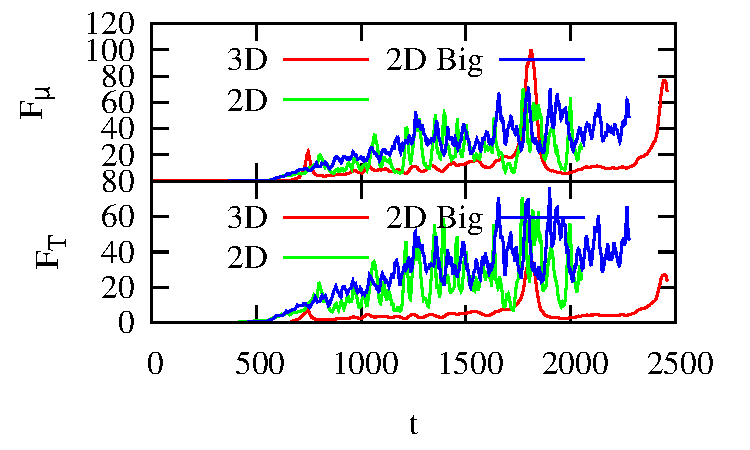
\includegraphics[width=0.35\textwidth]{figs/Pr=0_03_t=0_3_R0-1=1_1.pdf}}} &
	\vtop{\null\hbox{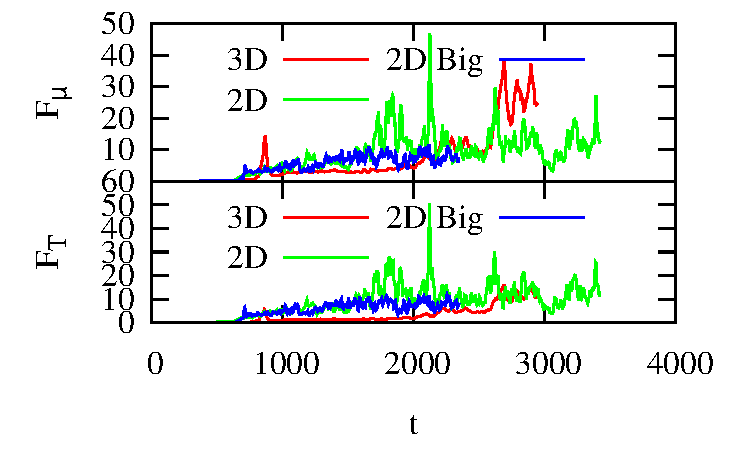
\includegraphics[width=0.35\textwidth]{figs/Pr=0_03_t=0_3_R0-1=1_2.pdf}}} \\
	\vtop{\null\hbox{\scalebox{0.7}{\begin{tabular}{r}
		$\rm{Pr}=0.01$ \\
		$\tau=0.01$ \\
		$R_{0}^{-1}=1.5,2$ \\
	\end{tabular}}}} &
	\fbox{\vtop{\null\hbox{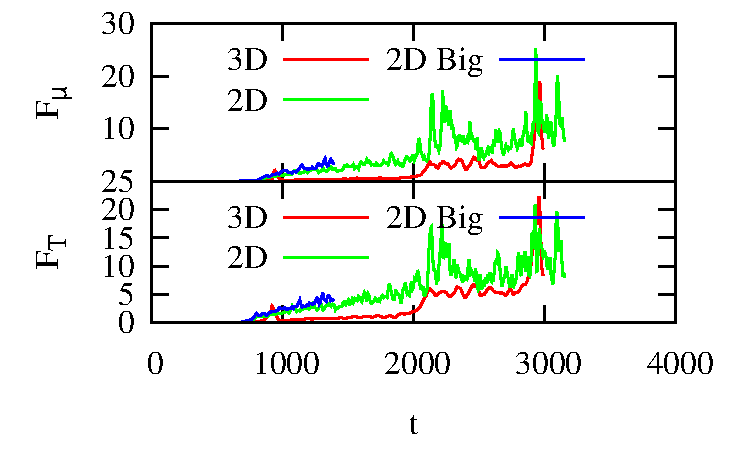
\includegraphics[width=0.35\textwidth]{figs/Pr=0_01_t=0_01_R0-1=1_5.pdf}}}} &
	\fbox{\vtop{\null\hbox{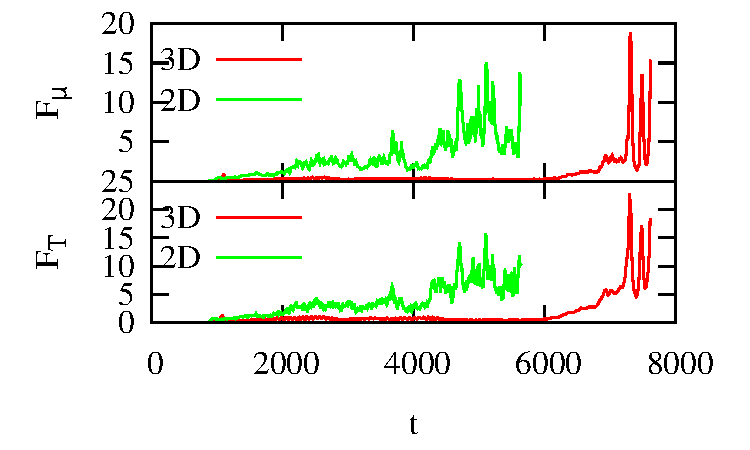
\includegraphics[width=0.35\textwidth]{figs/Pr=0_01_t=0_01_R0-1=2.pdf}}}} \\
\end{tabular}
}

\frame{\frametitle{These simulations show no sign of the strong horizontal shear apparent in the simulations at higher viscosity.}
\begin{figure}[h]
	\centering
		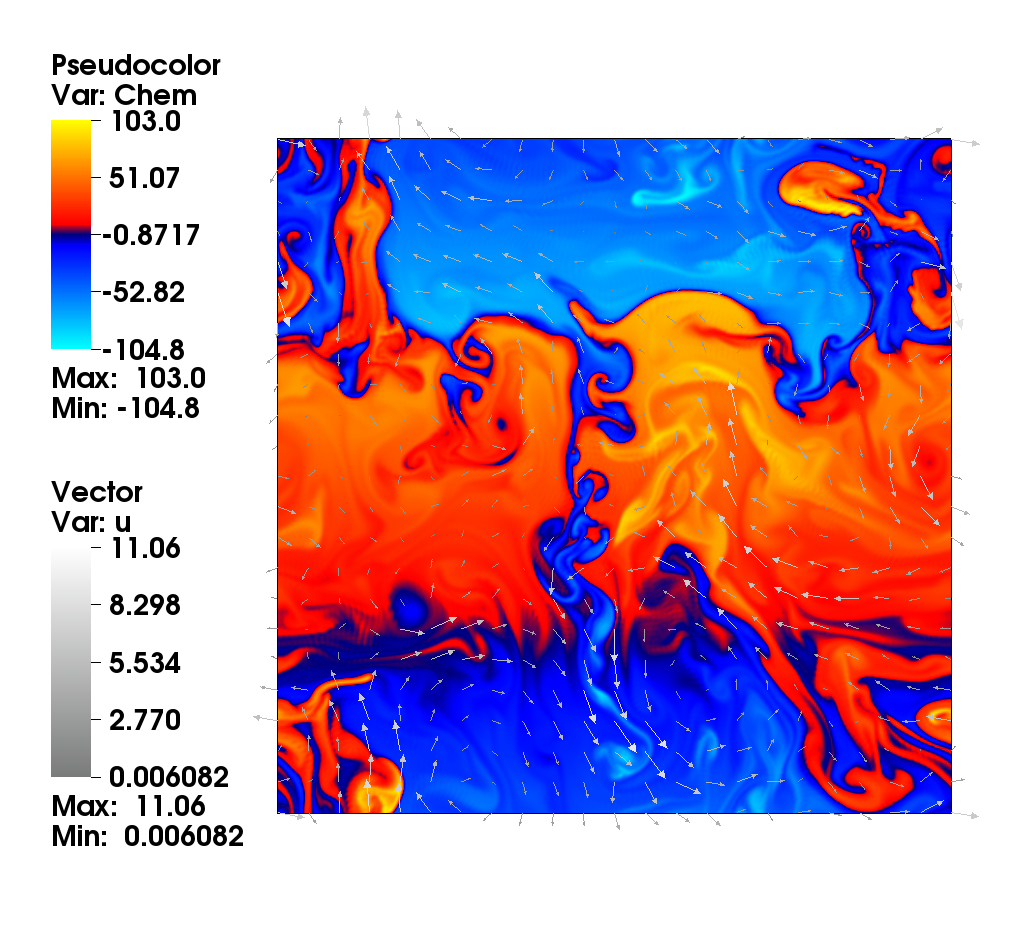
\includegraphics[width=.55\textwidth]{../pngs/sc_layers_0-03_0-03.png}
	\caption{$\rm{Pr}=0.03$, $\tau=0.03$, $R_{0}^{-1}=1.5$}
	\label{fig:pngs_sc_layers_0-03_0-03}
\end{figure}
}

% \subsection{Layered Semi-Convection}

% \frame{\frametitle{Future Code Development}
% \begin{itemize}
% 	\item Implement nonlinear diffusion (working in 1D) in 2D
% 	\begin{itemize}
% 		\item Examine layer properties with $\mu$-dependent diffusion
% 	\end{itemize}
% 	\item Upgrade from Boussinesq to Pseudo-Incompressible
% 	\begin{itemize}
% 		\item Determine layer height across density scale heights
% 	\end{itemize}
% 	\item Update KEPLER and MESA with layer height
% \end{itemize}}

% \subsection{Additional Slides}

% \frame{\tableofcontents[currentsubsection]}

% \subsubsection{Pseudo-Incompressibility}

% \frame{\frametitle{Governing equations}
% \begin{overprint}
% 	\only<1>{\bf Fully Compressible}
% 	\only<2>{\bf Incompressible, Current Equations}
% 	\only<3>{\bf Pseudo-Incompressible}
% 	% \only<4>{\bf Pseudo-Incompressible, Energy Conserving (Wood, private communication)}
% 	\only<1>{
% 	\begin{align}
% 		\rho\frac{D}{D{t}}{\mathbf{u}} =& -\nabla p + \rho \mathbf{g} + \nabla\cdot\mathbf{\Pi} \\
% 		\frac{D}{D{t}}\rho =& -\rho\nabla\cdot\mathbf{u} \\
% 		\rho{T}\frac{D}{D{t}}{s} =& \nabla\vect{u}:\vect{\Pi} + \sum_{i}\mu_{i}\nabla\cdot\vect{C}_{i} - \nabla\cdot{\vect{H}} \\
% 		\rho\frac{D}{D{t}}{\xi_{i}}=&-\nabla\cdot\vect{C}_{i}
% 	\end{align}}
% 	\only<2>{
% 	\begin{align}
% 		\rho_{0}\frac{D}{D{t}}{\mathbf{u}} =& -\nabla p + \left(-\alpha{T}+\beta\mu\right)\rho_{0}\mathbf{g} + \nu\rho_{0}\nabla^{2}\mathbf{u} \\
% 		\nabla\cdot\mathbf{u} =& 0 \\
% 		\frac{D}{D{t}}{T} + w\frac{d}{dz}T_{0} =& \kappa_T \nabla^{2}T \\
% 		\frac{D}{D{t}}{\xi_{i}} + w\frac{d}{dz}\xi_{i,0}=& \kappa_{i}\nabla^{2}\xi_{i}
% 	\end{align}}
% 	\only<3>{
% 	\begin{align}
% 		\rho\frac{D}{D{t}}\mathbf{u}=&-\nabla\left(p_{0}+p_{1}\right)+\frac{p_{1}}{\rho}\left(\frac{\partial p}{\partial \rho}\right)^{-1}\nabla p_{0} -\rho\nabla\Phi+\nabla\cdot\mathbf{\Pi}\\
% 		p_{0}\left(z\right)=&p\left(\rho,s,\xi_{1},\xi_{2},\dots\right)\\
% 		\frac{D}{D{t}}\rho =& -\rho\nabla\cdot\mathbf{u} \\
% 		\rho{T}\frac{D}{D{t}}{s} =& \nabla\mathbf{u}:\mathbf{\Pi} + \sum_{i}\mu_{i}\nabla\cdot\mathbf{C}_{i} - \nabla\cdot{\mathbf{H}}\\
% 		\rho\frac{D}{D{t}}\xi_{i}=&-\nabla\cdot\mathbf{C}_{i}, 
% 		% \only<4>{\left(T,\mu_{i}\right)\equiv\left(\frac{\partial e}{\partial s},\frac{\partial e}{\partial \xi_{i}}\right)+p_{1}\frac{\partial{\left(\frac{\partial e}{\partial s},\frac{\partial e}{\partial \xi_{i}}\right)}/\partial{\rho}}{\partial{p}/\partial{\rho}}}
% 	\end{align}}
% \end{overprint}
% }

% \frame{\frametitle{Incompressible Non-Dimensionalization}
% 	\begin{align}
% 		\frac{D}{D{t}}{\mathbf{u}} =& -\nabla p + \frac{-\mathrm{Ra}_{T}T+\mathrm{Ra}_{\mu}\mu}{\mathrm{Pr}} + \nabla^{2}\mathbf{u} \\
% 		\nabla\cdot\mathbf{u} =& 0 \\
% 		\frac{D}{D{t}}{T} =& \nabla\cdot\left(\mathrm{Pr}^{-1}+\frac{\kappa_{T,1}}{\nu}\left(z\right)\right) \nabla T \\
% 		\frac{D}{D{t}}{\xi_{i}} =& \frac{\tau}{\mathrm{Pr}}\nabla^{2}\xi_{i}
% 	\end{align}
% }

% \frame{\frametitle{To solve these equations, we choose the equation of state of an ideal mixture.}
% 	\begin{align}
% 		\rho\frac{D}{D{t}}\mathbf{u}=&-\nabla\left(p_{0}+p_{1}\right)+\frac{p_{1}}{\gamma p_{0}}\nabla p_{0} -\rho\nabla\Phi+\nabla\cdot\mathbf{\Pi}\\
% 		p_{0}\left(z\right)=&\frac{k\rho\tilde{T}}{\overline{m}}\\
% 		\frac{D}{D{t}}\rho =& -\rho\nabla\cdot\mathbf{u} \\
% 		\rho{T}\frac{D}{D{t}}{s} =& \nabla\mathbf{u}:\mathbf{\Pi} + \sum_{i}\mu_{i}\nabla\cdot\mathbf{C}_{i} - \nabla\cdot{\mathbf{H}}\\
% 		\rho\frac{D}{D{t}}\xi_{i}=&-\nabla\cdot\mathbf{C}_{i}, \left(T,\mu_{i}\right)\equiv\frac{c_{p}p_{0}+kp_{1}}{c_{p}p_{0}}\left(\tilde{T},\tilde{\mu_{i}}\right)
% 	\end{align}
% }

% \frame{\frametitle{We can simplify this by expressing the entropy equation as a temperature equation.}
% \begin{overprint}
% 	\only<1>{
% 		\begin{equation}
% 			\frac{D}{Dt}T=\frac{\partial T}{\partial \rho}\frac{D}{Dt}\rho + \frac{\partial T}{\partial s}\frac{D}{Dt}s + \frac{\partial T}{\partial \xi_{i}}\frac{D}{Dt}\xi_{i}.
% 		\end{equation}
% 		We can use the remainder of the governing equations and the equation of state to get the full equation.
% 	}
% 	\only<2>{
% 		\begin{equation}
% 			\rho\frac{D}{Dt}T=-\left(\gamma - 1\right)\rho T\nabla\cdot{u} + \left(\gamma - 1\right)\frac{\overline{m}}{k}\left(\nabla\vect{u}:\vect{\Pi}-\nabla\cdot{\vect{H}}\right).
% 		\end{equation}
% 	}
% \end{overprint}
% }

% \frame{\frametitle{Governing Equations}
% 	\begin{align}
% 		p_{0} &= \frac{\rho T}{\overline{m}} \\
% 		\rho\frac{D}{Dt}\vect{u} &= -\nabla\left(p_{0} + p_{1}\right) + \frac{p_{1}}{\gamma p_{0}}\nabla{p_{0}} - \rho \hat{y} + \nabla \cdot \vect{\Pi} \\
% 		\rho\frac{D}{Dt}\xi &= \nabla \cdot \rho \tau \nabla \xi \\
% 		\frac{1}{\gamma - 1}\rho\frac{D}{Dt} T &= -\rho T \nabla \cdot \vect{u} + \overline{m}\left(\nabla\vect{u}:\vect{\Pi} + \nabla\cdot \frac{\rho}{\overline{m}}\nabla{T}\right)\left(1 + Q\right) \\
% 		\nabla\cdot{p_{0}^{\frac{1}{\gamma}}} &= \frac{\gamma - 1}{\gamma}p_{0}^{\frac{1}{\gamma}-1}\left(\nabla\vect{u}:\vect{\Pi}-\nabla\cdot \frac{\rho}{\overline{m}}\nabla{T}\right)\left(1 + Q\right) \\
% 		\Pi_{ij} &= \rho \mathrm{Pr}\left(\frac{\partial u_{i}}{\partial x_{j}} + \frac{\partial u_{j}}{\partial x_{i}} - \frac{2}{3}\delta_{ij}\nabla\cdot{\vect{u}}\right)
% 	\end{align}
% }

% \subsubsection{Two-Component Ideal Mixture}

% \frame{\frametitle{Derivation of the Equation of State for a two-component mixture.}
% \begin{overprint}
% 	\only<1>{
% 	Start with the EOS for an ideal gas:
% 	\begin{align}
% 		e_{i}\left(\rho_{i},s_{i}\right)=&\frac{c_{V}}{m_{i}}\left(\frac{\rho_{i}}{m_{i}}\phi_{i} e^{\frac{m_{i}s_{i}}{k}}\right)^{\frac{k}{c_{V}}}
% 	\end{align}
% 	Each component of the gas must follow this, and the total energy is $\overline{m}e=m_{1}e_{1}+m_{2}e_{2}$.
% 	}
% 	\only<2>{
% 	Note the entropy of the mixture is defined as $\overline{m}s=m_{1}\xi_{1}s_{1}+_{2}\xi_{2}s_{2}-k\xi_{1}\ln{\xi_{1}}-k\xi_{2}\ln{\xi_{2}}$.
% 	We assume the gases are thermally coupled:
% 	\begin{align}
% 		T=&\left(\frac{\rho\xi_{1}\phi_{1}}{\overline{m}}e^{\frac{m_{1}s_{1}}{k}}\right)^{\frac{k}{c_{v}}}=\left(\frac{\rho\xi_{2}\phi_{2}}{\overline{m}}e^{\frac{m_{2}s_{2}}{k}}\right)^{\frac{k}{c_{v}}}\\
% 		e^{\frac{m_{1}s_{1}}{k}}=&\left(\frac{\xi_{2}\phi_{2}}{\xi_{1}\phi_{1}}\right)^{\xi_{2}}e^{\frac{\overline{m}s}{k}+\xi_{1}\ln{\xi_{1}}+\xi_{2}\ln{\xi_{2}}}
% 	\end{align}
% 	And likewise for $s_{2}$
% 	}
% 	\only<3>{
% 	Thus, the total energy is
% \begin{align}
% 	e_{1}\left(\rho,s,\xi_{1},\xi_{2}\right)&=c_{V}\left(\frac{\rho\xi_{1}\phi_{1}}{m_{1}}\left[\frac{\xi_{2}\phi_{2}}{\xi_{1}\phi{1}}\right]^{\xi_{2}} e^{\frac{\overline{m}s}{k}+\xi_{1}\ln{\xi_{1}}+\xi_{2}\ln{\xi_{2}}}\right)^{\frac{k}{c_{V}}},\\
% 	e_{2}\left(\rho,s,\xi_{1},\xi_{2}\right)&=c_{V}\left(\frac{\rho\xi_{2}\phi_{2}}{m_{2}}\left[\frac{\xi_{1}\phi_{1}}{\xi_{2}\phi{2}}\right]^{\xi_{1}} e^{\frac{\overline{m}s}{k}+\xi_{1}\ln{\xi_{1}}+\xi_{2}\ln{\xi_{2}}}\right)^{\frac{k}{c_{V}}},\\
% 	\overline{m} e\left(\rho,s,\xi_{1}\right)&=\sum_{i} m_{i} \xi_{i} e_{i}\left(\rho,s,\xi_{1},1-\xi_{1}\right).
% \end{align}
% 	}
% 	\only<4>{
% 	\begin{tabular}{|r | c | c | c |}
% 		\hline
% 		 & & $\frac{\partial}{\partial \rho}$ & $\frac{\partial/\partial \rho}{\partial p / \partial \rho}$ \\ \hline
% 		$p$ & $\frac{k}{c_{v}}\rho e$ & $\frac{c_{p}}{c_{v}}\frac{p}{\rho}$ & 1 \\ \hline
% 		$T$ & $\frac{e}{c_{v}}$ & $\frac{kT}{c_{v}\rho}$ & $\frac{kT}{c_{p}p}$ \\ \hline
% 		$\mu_{1}$ & $\frac{\frac{1}{\xi_{1}}\left(m_{2}-\overline{m}\right)\left(c_{p}-\overline{m}s\right)+k\ln{\frac{\phi_{1}}{\phi_{2}}}}{c_{v}}e$ & $\frac{k\mu_{1}}{c_{v}\rho}$ & $\frac{k\mu_{1}}{c_{p}p}$ \\ \hline
% 	\end{tabular}
% 	}
% \end{overprint}
% }